% Slides for 2024-07-09
% To create a slide, use the following:
\begin{frame}{Template matching}
    \centering
    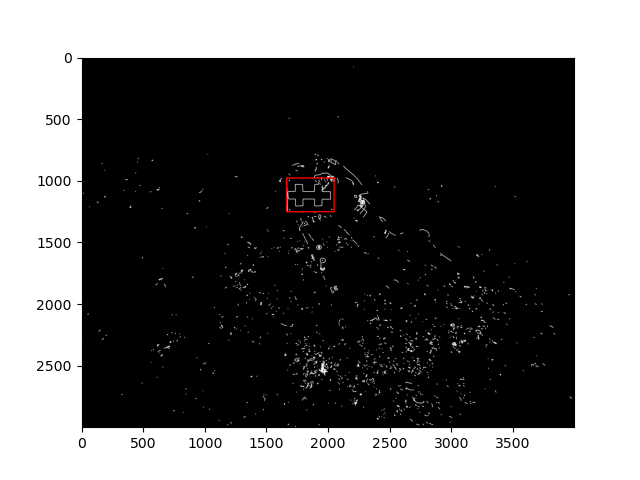
\includegraphics[height=0.6\textheight,width=0.6\textwidth,keepaspectratio]{images/fs_rectangle_contours.png}
    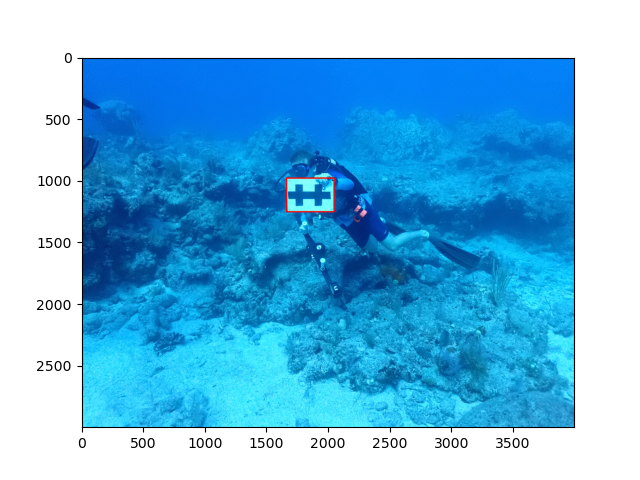
\includegraphics[height=0.6\textheight,width=0.6\textwidth,keepaspectratio]{images/fs_rectangle_real.png}
\end{frame}

\begin{frame}{Matching slate}
    \centering
    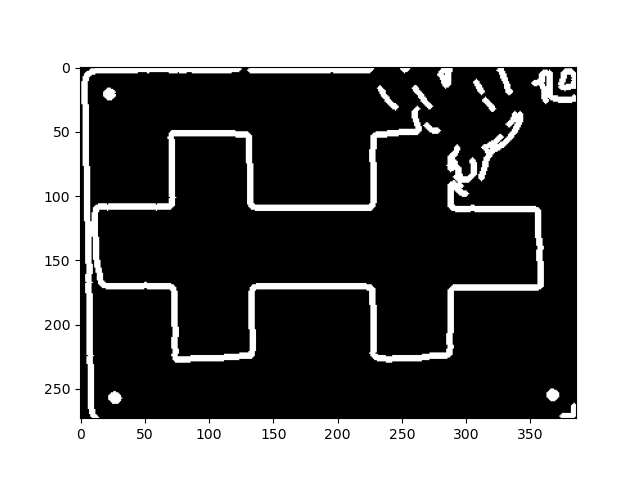
\includegraphics[height=0.7\textheight,width=0.7\textwidth,keepaspectratio]{images/fs_contours_cropped.png}
\end{frame}

\begin{frame}{FishSense Mobile}
    \begin{columns}
        \begin{column}{0.5\textwidth}
            \begin{itemize}
                \item UI/UX designs
                \item SQLite
            \end{itemize}
        \end{column}
        \begin{column}{0.5\textwidth}
            \centering
            
\includegraphics[height=0.7\textheight,width=0.7\textwidth,keepaspectratio]{images/fs_icons.png}
        \end{column}
    \end{columns}
\end{frame}

\begin{frame}{FishSense Mobile - Data Download}
    \begin{enumerate}
        \item Need to download data from apps
        \item dutchcoders/transfer.sh seems to be the easiest way to do this
    \end{enumerate}
\end{frame}

% To create a slide with a bullet list, use the following:
% \begin{frame}{TITLE}
%     \begin{itemize}
%         \item ITEM 1
%         \item ITEM 2
%     \end{itemize}    
% \end{frame}

% To create a slide with numbered list, use the following:
% \begin{frame}{TITLE}
%     \begin{enumerate}
%         \item ITEM 1
%         \item ITEM 2
%     \end{enumerate}
% \end{frame}

% To create a slide with a graphic:
% 1. Add the graphic to this folder (named picture.png)
% 2. Use the following:
% \begin{frame}{TITLE}
%     \centering
%     \includegraphics[height=0.7\textheight,width=0.7\textwidth,keepaspectratio]{picture.png}
% \end{frame}

% To create a slide with two columns, use the following:
% \begin{frame}{TITLE}
%     \begin{columns}
%         \begin{column}{0.5\textwidth}
%             COLUMN 1 BODY
%         \end{column}
%         \begin{column}{0.5\textwidth}
%             COLUMN 2 BODY
%         \end{column}
%     \end{columns}
% \end{frame}
